\multiproblem{methods}{Let's warm up by having a quick practice at finding the general solution for a couple of ODEs.
\begin{enumerate}
 \item Use the method of direct integration to find the set of solutions that solve
 \begin{equation}\label{eq:meth1}
  \frac{\dd x}{\dd t}=3t^{2}.
 \end{equation}
 On a single graph sketch the particular solutions of the initial value problem consisting of ODE \eqref{eq:meth1} with initial conditions $x(0)=x_{0}$, where
 \begin{enumerate}
  \item $x_{0}=0$
  \item $x_{0}=1$
  \item $x_{0}=-1$.
 \end{enumerate}
Now on the same graph sketch the particular solutions when $\frac{\dd x}{\dd t}=-3t^{2}$. What is the solution to the initial value problem given by  \eqref{eq:meth1} and initial condition $x(0)=x_{0}$, $x_{0}\in \mathbb{R}$?
 
 \item Use the method of separation of variables to find the set of solutions that solve
 \begin{equation*}\label{eq:meth2}
  \frac{\dd x}{\dd t}=2xt.
 \end{equation*}
On a single graph sketch the particular solutions of the initial value problem consisting of ODE \eqref{eq:meth2} with initial conditions $x(0)=x_{0}$, where
 \begin{enumerate}
   \item $x_{0}=0$
  \item $x_{0}=1$
  \item $x_{0}=2$
 \end{enumerate}
 Now on the same graph sketch the particular solutions when $\frac{\dd x}{\dd t}=-2xt$. What is the solution to the initial value problem given by  \eqref{eq:meth2} and initial condition $x(0)=x_{0}$, $x_{0}\in \mathbb{R}$?
\end{enumerate}
}

\multiproblem{rabbit}{Consider again the rabbit example that is given in the preamble. Some foxes escaped from a passing ship so the island is no longer a rabbit utopia. The rate of change of the rabbit population is now approximated by the following model
\begin{equation*}
 \frac{\dd N}{\dd t} = b N - d N
\end{equation*}
where $b$ represents the birth rate of rabbits and $d$ represents the death rate.
\begin{enumerate}
 \item Suppose some biologists arrived on the island and monitored the rabbit population. When they first arrived they counted four rabbits, and after 2 years there were 218. Assuming that the birth rate $b$ remains at 4, what is the death rate?
 \item Let $b-d=1.5$. For initial conditions $N(0)=3$, $N(0)=4$ and $N(0)=5$, how many rabbits are there after three months (approximate to the nearest rabbit)? Sketch the solution curves.
  \item Let $b-d=-1$. For initial conditions $N(0)=3$, $N(0)=4$ and $N(0)=5$, how many rabbits are there after three months (approximate to the nearest rabbit)? Sketch the solution curves.
  \item What happens when $b-d=0$ i.e. the birth rate is the same as the death rate? For initial conditions $N(0)=3$, $N(0)=4$ and $N(0)=5$, how many rabbits are there after three months? Sketch the solution curves.
  
\end{enumerate}
}

\multiproblem{tank}{Consider the problem of water flowing out of a tank introduced in the lectures.
        \begin{center}
        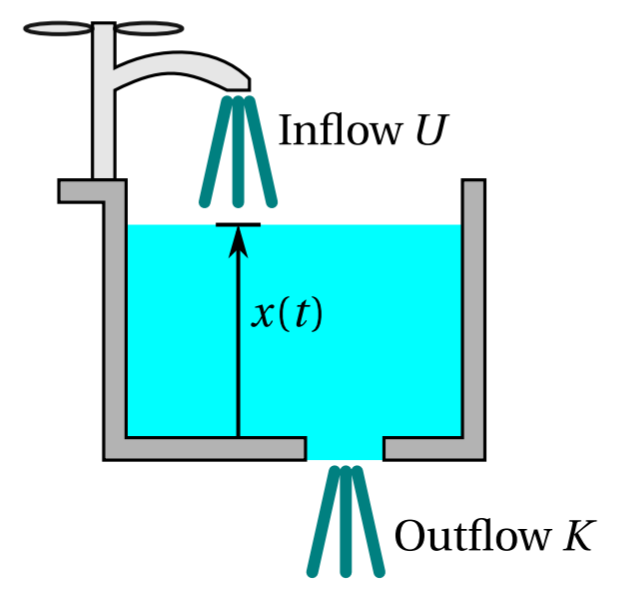
\includegraphics[scale=0.35]{tank.pdf}
        \end{center}
        Assume that there is no inflow to the tank, and that the outflow is given by Bernoulli's principle as $A\sqrt{2gx}$. Therefore the rate of change of the water level of the tank is given by the following ODE 
        \begin{equation}\label{eq:tank}
         \frac{\dd x}{\dd t}=-A \sqrt{2gx}
        \end{equation}
        where $A$ and $g$ are both constant.
        \begin{enumerate}
        \item By using the method of separation of variables, show that the solution to the ODE \eqref{eq:tank} is given by 
  \begin{equation*}
  x(t)=\alpha(D-t)^{2}\hspace{10pt}\text{where}\hspace{10pt}\alpha=\frac{A^{2}g}{2}>0,~~D=\frac{C}{A\sqrt{2g}}
  \end{equation*}
  and $C$ is the integration constant. Note that $\alpha$ is a constant greater than zero, whilst $D$ will change depending on the initial conditions. Sketch the solution curves for $D=-2,-1,0,1,2$. Notice that these curves intersect! At these points of intersection there are two possible solutions that satisfy \eqref{eq:tank}.
         \item Suppose that the tank is initially full to $x(0)=\alpha$. There are two possible solutions to this initial value problem. Find them and sketch them on a graph. By considering the sign of the rate of change of $x$ given in \eqref{eq:tank} explain why we can ignore the solution curve with a positive gradient at $x(0)=\alpha$. What would this spurious solution represent physically in terms of the water in the tank?
         \item Now just consider the reasonable solution with the negative gradient. Show that according to this solution, the tank becomes empty at time $t=D$. From looking at your sketch, what does the solution curve predict will happen afterwards? By considering what \eqref{eq:tank} tells you about $\frac{\dd x}{\dd t}$ at $x=0$ explain why it is not reasonable to follow the solution curve. Also, explain why it is not reasonable from thinking about what is happening to the water level in the tank physically. So what do you think happens at $t=0$?
         \item Show that for any arbitrary initial condition $x(t_{0})=x_{0}>0$ (the water in the tank cannot be at a negative distance from the bottom!) the value of $D$ corresponding to the solution that we choose with negative gradient is given by
\begin{equation}\label{eq:ddef}
 D=t_{0} + \sqrt{\frac{x_{0}}{\alpha}}.
\end{equation}
Hence convince yourself that for an arbitrary initial condition $x(t_{0})=x_{0}>0$ the unique solution is therefore given by
\begin{equation*}
 x(t)=\begin{cases}
       \alpha(D-t)^{2} & t\leq D \\
       0 & t>D.
      \end{cases}
\end{equation*}
where $D$ is defined as in \eqref{eq:ddef}. Sketch this unique solution for initial conditions $x(0)=\alpha$, $x(0)=4\alpha$, $x(1)=\alpha$ and $x(1)=4\alpha$.
         \end{enumerate}
}

\multiproblem{rabbit2}{
Back on rabbit island after some research the scientists camped on the island decide that the rate of change of the number of rabbits is actually best described by the ODE
\begin{equation}\label{eq:rabbit2}
 \frac{\dd N}{\dd t} = (b-d)N^{2}.
\end{equation}
\begin{enumerate}
 \item Assume more rabbits are being born than dying with $b-d=1$. Use separation of variables to show that in this case the solution is given by
\begin{equation*}
 N(t)=-\frac{1}{t+C}
\end{equation*}
where $C$ is the constant of integration.
 \item Suppose that there are four rabbits initially, so $N(0)=4$. Find and sketch the particular solution to the initial value problem made up of this initial condition and the ODE \eqref{eq:rabbit2}. 
 \item What happens where $t=1/4$? Does the model seem to make reasonable predictions after this point, i.e. for $t>\frac{1}{4}$?
 \item For an arbitrary initial condition i.e. an arbitrary number of rabbits at a arbitrary time (specifically $N(t_{0})=N_{0}$) what is the range of $t$ for which the model makes reasonable predictions?
 \item Can we find a solution to the initial value problem of \eqref{eq:rabbit2} with an initial condition that satisfies $N_{0}=0$ (for any $t_{0}$)? 
\end{enumerate}
}

\multiproblem{geom}{Consider the geometric equation given in the lectures
\begin{equation}\label{eq:geom}
 \frac{\dd x}{\dd t}=\frac{3x}{t}.
\end{equation}
\begin{enumerate}
 \item By using separation of variables show that solutions to this ODE are given by
 \begin{equation*}
  x(t)=At^{3}
 \end{equation*}
where $A \in \mathbb{R}$. Sketch the solutions for $A=-2,-1,0,1,2$.
\item By writing $A$ as a function of $x_{0}$ and $t_{0}$ for an arbitrary initial condition $x(t_{0})=x_{0}$, show that it is impossible to choose $A$ to satisfy an initial condition with $t_{0}=0$ and $x_{0}\neq 0$.
\item Is it possible to find a unique solution to the initial value problem of the ODE \eqref{eq:geom} with initial conditions $t_{0}=0$ and $x_{0}=0$? Explain why this is by referring to your earlier sketch.
\item For the initial value problem of ODE \eqref{eq:geom} with initial conditions $t_{0}>0$ do we have unique solution? What about for $t_{0}<0$? Hence determine the range of $t_{0}$ for which we have can have initial value problems with a unique solution. What happens to these solutions if they approach the origin (in the $x-t$ plane)?
\end{enumerate}
}

\multiproblem{unique}{
In the last three questions we have found that for certain values of initial conditions it has been impossible to find a unique particular solution to the initial value problem. Fortunately there is a useful theorem that tells us whether the solution we have found to an ODE will always give unique particular solution.

{\bf Uniqueness Theorem}\\
In general the solution $y(t)$ of an ODE
\begin{equation*}
 \frac{\dd x}{\dd t}=f(x,t)
\end{equation*}
is {\em unique} if (i) $|f(y,t)|<\infty$ and (ii) $|f_{x}(y,t)|<\infty$ for all $t$.\\

Let's consider the last question as an example to explain how you can apply this theorem to see if a solution to the ODE will be unique. The solution $y(t)$ is given by
\begin{equation*}
 y(t)=At^{3}.
\end{equation*}
Now we need to plug in this solution to the RHS of our ODE \label{eq:geom} to test the uniqueness conditions. We have
\begin{equation*}
 f(x,t)=\frac{3x}{t} \implies f(y,t)=\frac{3y}{t}=\frac{3At^{3}}{t}=3At^{2}.
\end{equation*}
Now because $|3At^{2}|<\infty$ for all $t<\infty$ condition (i) is satisfied. To test the second condition we first calculate 
\begin{equation*}
 f_{x}(x,t)=\frac{\partial }{\partial x} f(x,t)= \frac{\partial }{\partial x} \frac{3x}{t} = \frac{3}{t}.
\end{equation*}
Now this time we do not need to substitute $y(t)$ in because $f_{x}(x,t)$ does not depend on $x$. But we can see that  $|f_{x}(y,t)|$ blows up when $t=0$ so condition (ii) is violated.

\begin{enumerate}
 \item Verify that the solution $x(t)=\alpha(D-t)^{2}$ to the ODE \eqref{eq:tank} breaks at least one of the conditions of the uniqueness theorem.
 \item Verify that the solution $N(t)=-\frac{1}{t+C}$ to the ODE \eqref{eq:rabbit2} breaks at least one of the conditions of the uniqueness theorem.
 \end{enumerate}
}

\multiproblem{sines}{Consider the second-order ODE
\begin{equation*}
 \frac{\dd^{2} x}{\dd t^{2}}= -9 x.
\end{equation*}
\begin{enumerate}
\item Verify that $x(t)=\sin(3t)$ is a solution.
\item Verify that $x(t)=A\sin(3t)$ is a solution.
\item Verify that $x(t)=\cos(3t)$ is a solution.
\item Verify that $x(t)=A\sin(3t)+B\cos(3t)$ is a solution. \begin{enumerate}
                                                             \item If $x(0)=0.5$ and $x'(0)=0$, find $A$ and $B$ and hence the particular solution.
                                                             \item Show that $x(t)=A\sin(3t)+B\cos(3t)$ is the general solution by finding $A$ and $B$ in terms of the arbitrary initial conditions $x(t_{0})=x_{0}$ and $x'(t_{0})=v_{0}$. Is the solution unique?
                                                             \item Show that $x(t)=A\sin(3t)+B\cos(3t)$ satisfies both conditions of the uniqueness theorem.
                                                            \end{enumerate}
                                                            \end{enumerate}
                                                            
}



\multiproblem{newton}{In the lectures you considered Newton's Law of Motion for an object, say an apple, falling under gravity. This is a second-order ODE given by
\begin{equation}\label{eq:newton}
 \frac{\dd ^{2} x}{\dd t^{2}}=-g.
\end{equation}
        \begin{center}
        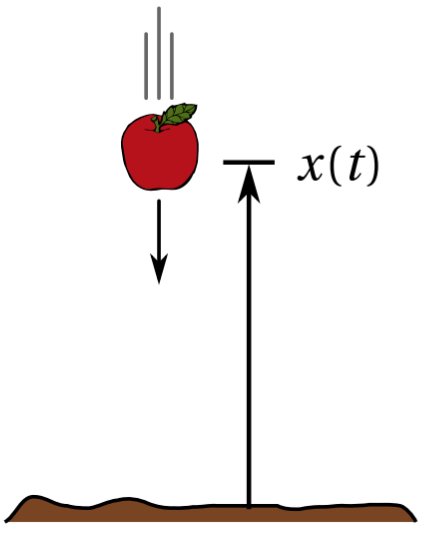
\includegraphics[scale=0.35]{newton.pdf}
        \end{center}
Here the position of the apple, denoted $x$, is our dependent variable and time $t$ is our independent variable. $x$ is defined to be pointing upwards away from the ground in the opposite direction to gravity $g$.
\begin{enumerate}
 \item Show that the solution found in lectures, 
 \begin{equation}\label{eq:newton_gen}
  x(t)=-\frac{gt^{2}}{2}+Ct+D,
 \end{equation}
satisfies the ODE \eqref{eq:newton}.
\item Suppose that our initial conditions are specified at time $t_{0} =0$, and are given by $x(0)=x_{0}$ and $x'(0)=v_{0}$. Find $C$ and $D$ in terms of $x_{0}$ and $v_{0}$. 
\item Take $g=10~\text{ms}^{-2}$. Suppose that the initial velocity $v_{0}=0$. Sketch the solution curves for $x_{0}=1$, $x_{0}=2$ and $x_{0}=3$.
\item Now suppose that the initial height $x(0)=5$. Sketch the solutions for $v_{0}=5~\text{ms}^{-1}$, $v_{0}=-5\text{ms}^{-1}$ and $v_{0}=0~\text{ms}^{-1}$. 
\item Suppose that after 2 seconds the apple has a velocity of $-5~\text{ms}^{-1}$ and is 12 m from the ground. What was position and velocity of the ball at time $t=0$? Sketch the solution.
\item Consider two arbitrary initial conditions, $x(t_{0})=x_{0}$ and $x'(t_{0})=v_{0}$. By finding $C$ and $D$ in terms of this arbitrary initial condition, show that \eqref{eq:newton_gen} is the general solution (can satisfy any initial condition). What does this imply about the uniqueness of the solutions?
 \end{enumerate}
}

